%This is chapter 2
%%=========================================
 \rhead{\itshape Internet des Objets}
\chapter{Internet des Objets}

\section{Introduction}
Le terme Internet des objets ou en anglais (Internet of Things) a été utilisé pour la première fois en 1990. Mais l’idée réelle d’appareils connectés existe depuis plus longtemps, du moins depuis les années 70. A l'époque, l'idée était souvent appelée "Internet embarqué" ou "informatique omniprésente". Le terme actuel «Internet of Things» a été inventé par Kevin Ashton en 1999 lors de son travail au centre MIT (Massachusetts Institute of Technology), qui travaillait à l’optimisation de la chaîne logistique, souhaitait attirer l’attention de la haute direction sur une nouvelle technologie passionnante appelée RFID. Parce qu’Internet était la nouvelle tendance la plus en vogue en 1999 et qu’il avait un sens, il a appelé sa présentation «Internet of Things».


Même si Kevin a suscité l’intérêt de certaines entreprises. Le terme Internet des objets n'a pas retenu l'attention au cours des dix prochaines années. Le terme Internet des objets a encore émergé à l'été 2010,  Selon des informations confidentielles, le service StreetView de Google n’avait pas seulement pris des photos à 360 degrés, il avait également stocké des tonnes de données sur les réseaux Wi-Fi de personnes. Les spécialistes se demandaient si c'était le début de la nouvelle stratégie de Google, non seulement pour l'indexation d'Internet, mais également pour l'indexée le monde physique.


La même année, le gouvernement chinois a annoncé qu'il ferait de l'Internet des objets une priorité stratégique de son plan quinquennal.


En 2011, Gartner, la société d’études de marché qui a inventé le fameux « hype-cycle for emerging technologies » a ajouté un nouveau phénomène émergent à sa liste: «l’Internet des objets». L’année suivante, le thème de la plus grande conférence Internet européenne, Le Web, était l’Internet des objets. Parallèlement, des magazines populaires axés sur la technologie, tels que Forbes, Fast Company et Wired, ont commencé à utiliser l'IoT comme vocabulaire pour décrire le phénomène.


En octobre 2013, International Data Corporation (IDC) a publié un rapport indiquant que l'Internet des objets représenterait un marché de 8 900 milliards de dollars en 2020.


Le terme Internet of Things a atteint la notoriété sur le marché de masse quand, en janvier 2014, Google a annoncé l'achat de Nest pour 3,2 milliards de dollars. Au même moment, le Consumer Electronics Show (CES) de Las Vegas s'est tenu sous le thème de l'IoT.


Actuellement, il y a plus de 26 milliards d'appareils IoT connectés, devrait dépasser 75 milliards en 2025. La valeur du marché mondial de l'IoT en 2019 dépasse 1,7 billion de dollars et le matériel représente 35\% de cette valeur.
\section{Internet  des objets}
L'objet connecté est un objet électronique qui peut  transmettre des informations en temps réel via une liaison sans fil à une autre dispositif connecté. Ces informations peuvent être de plusieurs types \cite{1} .


Les objets connectés sont des équipements du quotidien qui dotés de capteurs et de dispositifs d’échange de données, permettent de disposer à distance d’informations sur une partie de notre environnement, ou échangent de l’information pour produire un service \cite{2,3}.


Un objet connecté est un matériel, disposant de composants électroniques lui permettant de communiquer des informations vers un autre objet, un serveur informatique, un ordinateur, une tablette ou un smartphone, en utilisant une liaison sans fil vers un réseau dédié (le plus souvent Internet) \cite{4}.


Un objet connecté tend aussi à avoir une capacité de traitement qui lui est propre sur les données qu’il capte ou mesure. Ce traitement local permettant d’alléger la quantité des informations transmises pour s’adapter à la capacité du lien de communication ou des systèmes de traitement distants \cite{5}. 


La capacité de traitement des objets connectés tend aussi à intégrer des logiques dites « intelligentes » c’est-à-dire capables d’agir sur le comportement \cite{6} de l’objet lui-même ou de moduler la transmission d’informations, en fonction des informations captées ou des mesures effectuées \cite{7}.


Un objet peut être  une entité physique ou virtuelle ayant des identités et des personnalités virtuelles, opérant dans des espaces intelligents et utilisant des interfaces intelligentes pour se connecter et communiquer au sein de contextes d’usages variés \cite{8}.

Lorsque qu’un ensemble d’objets connectés communiquent et interagissent entre eux ou avec des serveurs de traitement via le réseau Internet, on parle alors d’Internet des Objets (IdO) ou Internet of Things (IoT).
\section{Architecture de l'internet des objets}
Dans l'IoT, chaque couche est définie par ses fonctions et les périphériques utilisés dans cette couche. L'architecture de l'IoT est généralement divisée en trois couches, la couche perception, la couche réseau et la couche application \cite{9}.

\begin{figure}[H]
\centering
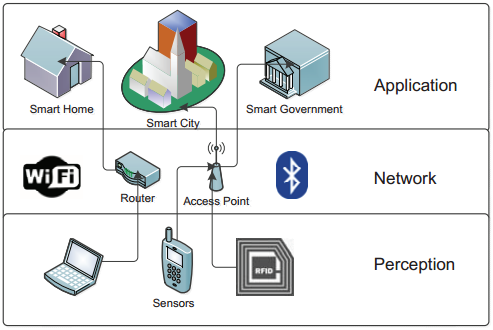
\includegraphics[scale=1]{chap1/fig1.png}
\caption{Architecture à trois couches de l'IoT \cite{10}}
\label{fig1}
\end{figure}
\subsection{Couche de perception}
La couche de perception est également connue sous le nom de couche «Capteurs» dans l'IoT. Le but de cette couche est d'acquérir les données de l'environnement à l'aide de capteurs et d'actionneurs. Cette couche détecte, collecte et traite les informations, puis les transmet à la couche réseau. Cette couche effectue également la collaboration des nœuds IoT dans les réseaux locaux et à courte porté \cite{11}.
\subsection{Couche réseau}
La couche réseau de l'IoT sert à la fonction de routage et de transmission des données vers différents hubs et appareils IoT sur Internet. À cette couche, les plates-formes de cloud computing, les passerelles Internet, les dispositifs de commutation et de routage ...etc. fonctionnent en utilisant certaines technologies très récentes telles que WiFi, LTE, Bluetooth, 3G, Zigbee, etc. Les passerelles réseau servent de médiateur entre différents IoT nœuds en agrégeant, filtrant et transmettant des données vers et depuis différents capteurs \cite{12}.
\subsection{Couche d'application}
La couche application est considérée comme une couche supérieure de l'architecture IoT conventionnelle. Cette couche fournit des services personnalisés en fonction des besoins des utilisateurs \cite{13}. La responsabilité principale de cette couche est de relier l'écart majeur entre les utilisateurs et les applications. Cette couche IoT combine l'industrie pour atteindre les solutions de type d'applications intelligentes de haut niveau telles que la surveillance des catastrophes, la surveillance de la santé, la transposition, la fortune, l'environnement médical et écologique et la gestion globale gérée pertinente pour toutes les applications de type intelligent.
\section{Objet connecté}
Un «objet» dans «l'Internet des objets» est une unité de traitement capable de se connecter à Internet et d'échanger des données avec le cloud. Les appareils sont souvent appelés «appareils intelligents» ou «appareils connectés». Ils communiquent deux types de données: la télémétrie et l'état \cite{zouganeli2009connected}.
\subsection{Types d'informations}Chaque appareil peut fournir ou consommer différents types d'informations. Chaque forme d'information peut être gérée au mieux par un système backend différent, et chaque système doit être spécialisé autour du débit de données, du volume et de l'API préférée.
\begin{enumerate}
       \item \textbf{Métadonnées de l'appareil :} les métadonnées contiennent des informations sur un périphérique. La plupart des métadonnées changent rarement, voire jamais. Exemples de champs de métadonnées  \cite{apthorpe2017smart}:
    \begin{itemize}
        \item Identifiant (ID)
        \item Classe ou type
        \item Modèle
        \item Révision
        \item Date de fabrication
        \item Numéro de série du matériel
    \end{itemize}
    \item \textbf{Télémétrie :} les données collectées par l'appareil sont appelées télémétrie. Ce sont les données des yeux et des oreilles que les appareils IoT fournissent aux applications. La télémétrie est une donnée en lecture seule sur l'environnement, généralement collectée via des capteurs \cite{satija2017real}.
    \item \textbf{Informations sur l'état :} les informations d'état décrivent l'état actuel de l'appareil, pas celui de l'environnement. Ces informations peuvent être lues / écrites, mis à jour, mais généralement pas fréquemment \cite{kim2015iot}.
    \item \textbf{Commandes de périphérique :} les commandes sont des actions effectuées par un appareil. Les commandes peuvent être valides pour une période de temps limitée, elles doivent donc inclure une durée de vie ou time to live (TTL)  en anglais ou une autre valeur d'expiration \cite{kim2015iot}.
    \item \textbf{Informations opérationnelles :} les informations opérationnelles sont les données les plus pertinentes pour le fonctionnement de l'appareil par opposition à l'application métier. Cela peut inclure des éléments tels que la température de fonctionnement du processeur et état de la batterie. Ce type de données peut ne pas avoir de valeur analytique à long terme, mais il a une valeur à court terme pour aider à maintenir l'état de fonctionnement, comme répondre aux pannes et corriger la dégradation des performances du logiciel après les mises à jour.Les informations opérationnelles peuvent être transmises sous forme de données de télémétrie ou d'état \cite{tang2019review}.

\end{enumerate}
\subsection{Types des objets connectés}
Il y a plusieurs critères de classification des types des objets, Il existe deux grandes modèles des objets connectés qui sont : 
\subsubsection{Les objets portés } De manière générale, les termes «technologie wearable», «dispositifs wearable» et «vêtements intelligents» se réfèrent tous à des technologies électroniques ou à des micro-ordinateurs qui sont incorporés dans des vêtements et des accessoires, qui peuvent être portés sur le corps. Suite au fait que les performances de calcul augmentent constamment, les objets portés contemporains deviennent capables d'effectuer des tâches informatiques similaires à celles des smartphone ou même des ordinateurs portables.
\subsubsection{Les objets indépendants} Tous les objets non portables avec des capteurs déployés à plusieurs endroits, comme les stations météos, les voitures intelligentes, les drones...etc

Il existe une autre classification pour déterminer les types des objets connecté, ils peuvent être classés en grande partie soit passifs soit actifs en fonction de la source d’énergie détectée.
\subsubsection{Les objets passifs} Utiliser généralement c’est un tag (carte pus, tag RFID, NFC, code barre) Les technologies de capteurs passifs collectent des données cibles grâce à la détection des vibrations, de la lumière, du rayonnement, de la température  ou d'autres phénomènes se produisant dans l'environnement.
\subsubsection{Les objets actifs} Un objet a une capacité de stockage et de traitement qui comprennent des émetteurs qui envoient un signal, une longueur d'onde lumineuse ou des électrons à rebondir sur la cible, avec des données recueillies par le capteur lors de leur réflexion.
\subsection{Capteurs et actionneurs}
Les capteurs sont les yeux et les oreilles de l'objet IoT pour voir son environnement, et les actionneurs sont les jambes et les mains qui remplissent ses fonctions.
\subsubsection{Capteurs}
Un capteur est un appareil qui convertit un paramètre physique en une sortie électrique. Un capteur est un type de transducteur. Les capteurs peuvent être divisés en capteurs analogiques et capteurs numériques. Les capteurs analogiques fournissent une sortie sous forme de tensions et de courants. Les microcontrôleurs auront besoin d'un ADC (analogue-to-digital converter) \cite{hoeschele1994analog} pour lire les données des capteurs analogiques. De nombreux capteurs plus récents sont des capteurs numériques \cite{kaltenbacher2007numerical}, c'est-à-dire qu'ils fournissent une sortie au format numérique, en utilisant des protocoles tels qu’I2C (Inter‐Integrated Circuit), SPI (Serial Peripheral Interface) \cite{marinkovic2011nano} et UART (universal asynchronous receiver/transmitter) \cite{chun2011universal}, etc. Les capteurs numériques sont excellents. Pour les systèmes embarqués, car ils contournent le besoin d'ADC et rendent le circuit beaucoup plus simple. Les exemples incluent les capteurs de température, les capteurs d'humidité, les capteurs de pression, les capteurs de fumée, les capteurs de son et de lumière, ..etc.



Il existe de nombreux capteurs disponibles pour l'IoT et un certain nombre de façons de les catégoriser. Les catégories décrites ci-dessous ne sont qu'un petit échantillon des façons dont les capteurs peuvent être regroupés. Les capteurs peuvent être divisés par:
\begin{enumerate}
    \item \textbf{leurs besoins en alimentation externe} \cite{stamatiadis2010comparison,messina2001integrated}:

% Please add the following required packages to your document preamble:
% \usepackage{booktabs}
\begin{table}[H]
\begin{tabular}{@{}|l|l|l|@{}}
\toprule
\textbf{Type}    & \multicolumn{1}{c|}{\textbf{Définition}}                                                                                                                & \multicolumn{1}{c|}{\textbf{Exemple}}                                                                                                       \\ \midrule
\textbf{Passive} & \begin{tabular}[c]{@{}l@{}}Ne nécessite pas d'alimentation externe \\ pour fonctionner. Ils répondent aux entrées de \\ leur environnement.\end{tabular} & \begin{tabular}[c]{@{}l@{}}Un capteur de température qui modifie \\ la résistance en réponse aux changements \\ de température\end{tabular} \\ \midrule
\textbf{Active}  & \begin{tabular}[c]{@{}l@{}}Nécessite une alimentation externe pour \\ fonctionner.\end{tabular}                                                         & une camera                                                                                                                                  \\ \bottomrule
\end{tabular}
\end{table}

\item \textbf{Type de signal produit par le capteur} \cite{eldar2012compressed,pallas2012sensors}:
% Please add the following required packages to your document preamble:
% \usepackage{booktabs}
\begin{table}[H]
\centering
\begin{tabular}{@{}|l|l|l|@{}}
\toprule
\textbf{Type}       & \textbf{Définition}                                                                                                                                & \textbf{Exemple}                                                                                           \\ \midrule
\textbf{Analogique} & Émet un signal analogique continu                                                                                                                  & \begin{tabular}[c]{@{}l@{}}Accéléromètres, \\ capteurs de température\end{tabular}                         \\ \midrule
\textbf{Numérique}  & \begin{tabular}[c]{@{}l@{}}La sortie est convertie en valeurs\\ discrètes (1s et 0s numériques) avant \\ de transmettre à un appareil\end{tabular} & \begin{tabular}[c]{@{}l@{}}Capteur de pression numérique,\\  capteur de température numérique\end{tabular} \\ \bottomrule
\end{tabular}
\end{table}

\item \textbf{Type d'appareil de mesure} \cite{homola1997sensitivity,pastre2010continuously,chen2017electronic}:

\begin{table}[H]
\begin{tabular}{|l|l|l|}
\hline
\textbf{Type}       & \textbf{Définition}                                       & \textbf{Exemple}   \\ \hline
\textbf{Chimique}   & Répond aux changements chimiques dans son environnement   & Capteur de gaz     \\ \hline
\textbf{mécanique}  & Répond aux changements physiques de son environnement     & Micro-interrupteur \\ \hline
\textbf{électrique} & Répond aux changements électriques dans son environnement & Capteur optique    \\ \hline
\end{tabular}
\end{table}
\end{enumerate}
Le choix des capteurs pour un projet nécessite une compréhension claire de ce qu'on veut mesurer  et de la précision requise.


Lors de la sélection d'un capteur IoT, plusieurs éléments doivent être pris en compte. En règle générale, l'objectif d'un capteur et d'un dispositif IoT est une longue durée de vie avec peu d'interaction humaine.Il faut placer les capteurs et appareils IoT dans l'environnement souhaité et pour les faire fonctionner pendant une période de temps prolongée. Ils peuvent se trouver dans un endroit éloigné ou être enfouis profondément dans un système, inaccessibles aux humains. Le remplacement d'un capteur et d'un appareil dans cette situation peut être extrêmement coûteux, dangereux, voire impossible; toutes les raisons de bien réfléchir aux décisions concernant le capteur et  appareil.


La décision est basée sur de nombreux facteurs. pour concerver le système, il faut soigneusement considérer l'importance de chaque facteur et sa priorité pour la conception globale.


La liste suivante de considérations peut être considérée comme un point de départ pour toute discussion sur les capteurs IoT:

\begin{itemize}
    \item \textbf{Durabilité :} la durabilité doit être prise en compte en ce qui concerne l'environnement du capteur. il faut assurer que l'appareil est aussi durable que nécessaire pour fonctionner pendant une période de temps raisonnable, sans encourir de coûts inutiles \cite{fedele2018energy}.
    
    
Par exemple, un capteur de température résistant à l'eau peut être acceptable pour une station météorologique à distance, mais il ne conviendrait pas du tout pour surveiller la température de l'eau dans une piscine car il n'est pas étanche.


\item \textbf{Précision :} afin d'avoir suffisamment de précision pour surveiller correctement un environnement, mais ne pas payer plus que ce dont on a besoin \cite{agarwal2016unified}.


Par exemple, concevez un système pour réguler la température dans une unité de stockage domestique à distance, il faut probablement être prêt  à accepter un capteur qui pourrait être précis avec +/- 2 degrés. Cette précision serait totalement inacceptable dans un système de dispositifs médicaux. Un capteur de température de dispositif médical devrait être précis à +/- 0,2 degré!

\item \textbf{Polyvalence :}  les capteurs doivent pouvoir fonctionner dans des variations raisonnables de l'environnement. Parce que la plupart des conceptions de réseaux IoT ont de nombreux capteurs, dans une variété d'environnements, il est important d'avoir des capteurs qui peuvent fonctionner avec précision dans toutes les variations de l'environnement \cite{santucci2010internet}.


Par exemple,pour construire des stations météorologiques éloignées pour les zones sauvages, On doit utiliser des capteurs capables de gérer les températures extrêmes d'été et d'hiver. Il ne serait pas pratique d'avoir des capteurs qui ne fonctionnent avec précision qu'à température ambiante.
\item \textbf{Consommation d'énergie : } selon la situation, les besoins peuvent concerner un périphérique à faible consommation, voire à très faible consommation. Il faut décider si des fonctions d'économie d'énergie (comme le mode veille ou le réveil rapide) sont nécessaires \cite{mainetti2011evolution}.


Par exemple, un capteur ou un appareil alimenté par des batteries solaires peut avoir besoin de passer une grande partie de sa vie en mode veille pour prolonger la durée de vie de la batterie pendant les périodes de faible éclairage. Il peut également nécessiter des temps de réveil rapides pour capturer avec précision les données.

\item \textbf{Considérations environnementales spéciales :} le choix du capteur peut même affecter la conception finale du système \cite{kelly2013towards}.


Par exemple, lors de la conception d'un système de surveillance de la qualité de l'eau, un capteur qui peut être placé dans la tuyauterie principale d'alimentation en eau est beaucoup plus rentable et précis qu'un capteur qui nécessite de détourner des échantillons d'eau.

\item \textbf{Coût :} les réseaux IoT impliquent généralement des centaines voire des milliers de capteurs et d'appareils. Tous les aspects de la conception des capteurs doivent être examinés du point de vue des coûts. Ces coûts impliquent plus que le prix du capteur. Il faut tenir compte du coût de placement, d'entretien, de fiabilité,..etc \cite{mhatre2005minimum}.
\end{itemize}

\subsubsection{Actionneur}
Un actionneur est un dispositif qui convertit un signal électrique en sortie physique \cite{wirtz2018brave}, c'est-à-dire un mouvement. Un actionneur peut être contrôlé par la tension ou le courant électrique, la pression pneumatique ou hydraulique \cite{arauz2013actuator}, ou même la puissance humaine. Dans les systèmes embarqués, les actionneurs sont principalement contrôlés par l'électricité. Lorsque le signal de commande est reçu, l'actionneur convertit l'énergie électrique en mouvement mécanique. Les actionneurs peuvent créer un mouvement linéaire, un mouvement rotatif ou un mouvement oscillatoire. Des exemples d'actionneurs comprennent les moteurs électriques, les actionneurs piézoélectriques, les actionneurs pneumatiques, les moteurs pas à pas et les actionneurs de serrure de porte, etc \cite{ham2009compliant}.
\subsection{Caractéristiques fondamentales de l'internet des objets}
Les caractéristiques fondamentales de l'IoT sont les suivantes :
\begin{enumerate}
    \item \textbf{Interconnexion :} il facilite l'interconnexion d'appareil et d'appareil à appareil \cite{fortino2018towards}.


\item \textbf{Détection intelligent :} les appareils connectés à l'IoT auront des capacités de détection intelligente. Par exemple, l'utilisation de détecteurs de mouvement pour allumer ou éteindre les lumières. La technologie de détection aide à créer des expériences qui reflètent une véritable conscience du monde physique, des personnes et des objets \cite{chen2017smart}.


\item \textbf{Intelligence :} les appareils connectés à l'IoT peuvent être dotés d'intelligence. Par exemple, les Nest Learning Thermostats sont compatibles Wi-Fi, pilotés par capteur et dotés de capacités d'auto-apprentissage. Le Misfit Shine est un tracker de fitness avec des capacités de surveillance du sommeil. Le Misfit Shine peut distribuer des tâches de calcul entre un smartphone et le cloud \cite{zhou2017computation}.


\item \textbf{Économiser l'énergie :} les appareils IoT comme Motion Sensor Light ont un détecteur de mouvement intégré qui peut allumer la lumière lorsqu'elle détecte un mouvement. Il peut économiser beaucoup d'énergie électrique du gaspillage et stimuler la récupération d'énergie et l'utilisation efficace de l'énergie  \cite{mainetti2011evolution}.


\item \textbf{Expressive :} les appareils connectés à l'IoT ont une capacité unique de dire l'état actuel aux autres appareils connectés dans les environs. Ils donnent un meilleur flux de communication entre l'homme et les machines \cite{odelu2017expressive}.


\item \textbf{Sécurisé :} les appareils connectés à l'IoT peuvent contribuer à garantir la sécurité de la vie individuelle. Par exemple, un pneu de voiture en mouvement peut indiquer son état actuel au propriétaire de la voiture ayant des tableaux de bord de voiture intelligents, cela aidera à prévenir les accidents dus à l'éclatement des pneus de voiture en raison d'une surchauffe,..etc \cite{naik2017cyber}.
\end{enumerate}
\subsection{Axes de l’internet des objets}
L'Internet des objets représente la troisième vague révolutionnaire de la technologie informatique après l'ordinateur personnel et Internet \cite{4}. Certains chercheurs considèrent l'IoT comme la prochaine phase de l'évolution d'Internet pour atteindre l'objectif de l'apprentissage machine à machine (M2M) \cite{8}. D'autres chercheurs considèrent l'IoT comme une extension du réseau Internet \cite{14}. Cependant, il existe une différence majeure entre l'IoT et Internet. Les sections suivantes mettent en évidence l'IoT et sa différence avec Internet.


L'IoT est différent d'Internet sur le plan de la communication. La communication Internet peut être établie à tout moment et en tout lieu. Cependant, la communication dans l'IoT a la dimension Any THING comme dimension supplémentaire, comme illustré la figure \ref{fig2} \cite{15}. L'objectif principal de l'IoT est de fournir une connectivité pour tout le monde à tout moment et en tout lieu.


Le concept IoT fonctionne pour unir et relier le monde physique et le monde virtuel \cite{4}, et le lien échange des données entre des appareils réels et des cyber-applications dans une connexion sécurisée \cite{16}. La forme physique de l'IoT se compose de périphériques externes, qui sont partagés au sein de l'infrastructure Internet \cite{17}. 

Cependant, certains appareils sont directement liés à l'IoT comme la RFID, les capteurs et les actionneurs qui comblent le fossé entre le monde physique et le monde de l'information \cite{18}. L'IoT relie différents types d'objets entre eux et leur permet de communiquer intelligemment \cite{19}. Une telle configuration atteint l'objectif d'identité, de suivi et de gestion intelligents \cite{4}

\begin{figure}[H]
\centering
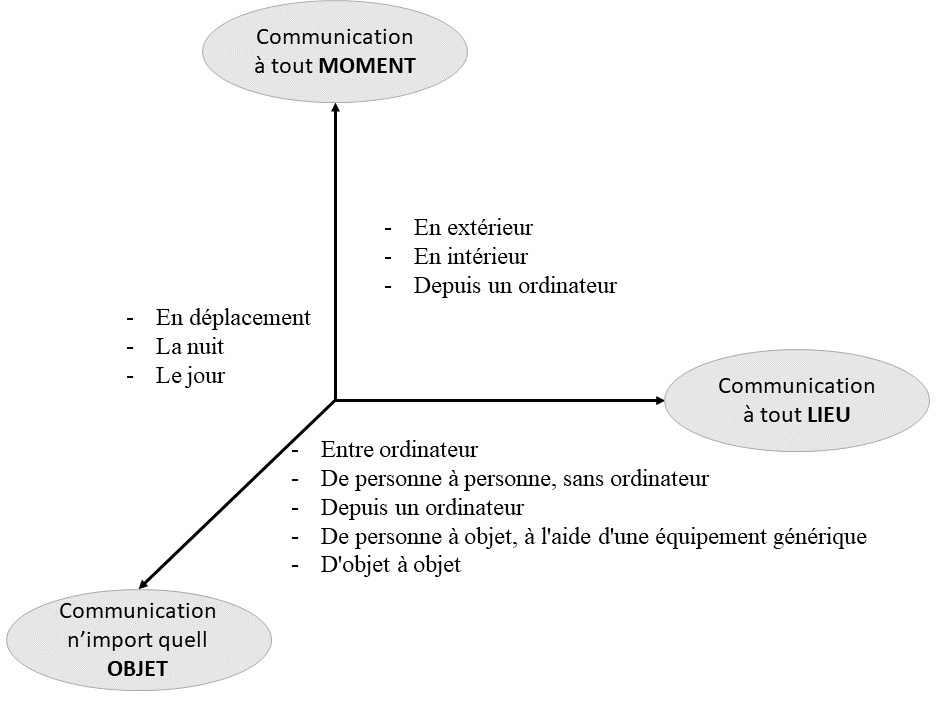
\includegraphics[scale=0.45]{chap1/Presentation2.png}
\caption{Axes de l’internet des objets \cite{10}}
\label{fig2}
\end{figure}

\section{Domaine d’application de l’internet des objets }
IoT est utilisé dans plusieurs domaines, nous citons comme exemples:
\subsection{Maison intelligente}
Les maisons intelligentes \cite{geneiatakis2017security} seront probablement les applications IoT les plus populaires. La maison intelligente, ou domotique, est une extension de l'automatisation du bâtiment, avec laquelle nous pouvons surveiller et contrôler le chauffage, la ventilation et la climatisation (CVC), l'éclairage \cite{yamamoto2012using}, les appareils électroménagers, les systèmes de sécurité à bande. En connectant tous les appareils électroménagers, nous pouvons automatiser de nombreuses routines quotidiennes, comme allumer et éteindre automatiquement les lumières et le chauffage, démarrer ou arrêter la cuisson et le lavage, etc. Avec le réseau intelligent et les compteurs intelligents, nous pouvons réduire les consommations d'énergie et les factures de services publics, et avec les systèmes de sécurité, nous pouvons rendre la maison plus sûre en détectant automatiquement et en dissuadant, espérons-le, les intrusions en utilisant divers capteurs infrarouges, de mouvement, sonores, de vibration ainsi que des systèmes d'alarme \cite{kodali2016iot}.


Une maison intelligente peut également rendre les personnes âgées et les personnes handicapées plus confortables et plus sûres à la maison. Avec l'IoT, nous pouvons collecter et analyser les données des personnes âgées et handicapées pour diagnostiquer les maladies, prédire les risques potentiels, identifier ou prévenir les accidents tels que les chutes, ouvrir ou verrouiller la porte (ou les fenêtres) à distance, et laisser les membres de la famille les surveiller à distance \cite{kodali2016iot}. Avec l'IoT, il est également possible de rapprocher les personnes âgées et handicapées du monde extérieur et de réduire leur sentiment de solitude.


Le marché de la maison intelligente devrait avoir une valeur marchande de plus de 53 milliards de dollars en 2022 \cite{sovacool2020smart,zhao2020analysis}.

\subsection{La santé}
L'IoT permet la surveillance à distance de la santé et les systèmes de notification d'urgence. Une approche très populaire consiste à utiliser des techniques portables. Ces appareils portables peuvent collecter une gamme de données de santé, telles que la fréquence cardiaque, la température corporelle et la pression artérielle, qui peuvent ensuite être transmises sans fil à un site distant pour le stockage et une analyse plus approfondie. Cela permet également à la télésanté/télémédecine, c'est-à-dire de diagnostiquer ou de traiter les patients à distance \cite{catarinucci2015iot}.
\subsection{Transport}
L'IoT peut considérablement améliorer les systèmes de transport. Avec toutes les voitures connectées, il est beaucoup plus facile de planifier votre voyage, d'éviter les embouteillages, de trouver une place de parking et de réduire les accidents de la circulation \cite{kong2017millimeter}. Les voitures sans conducteur auront sans aucun doute le plus grand impact. De nombreuses entreprises, telles que Tesla, Google, Über, Volvo, Volkswagen, Audi et General Motors, les développent et les promeuvent activement. Les voitures sans conducteur peuvent rendre notre voyage plus agréable et peut-être beaucoup plus sûr. Obtenir un permis de conduire pourrait bientôt être chose du passé \cite{petrov2017vehicle}

L'IoT peut également bénéficier aux transports publics. En connectant tous les panneaux d'information et les panneaux publicitaires dans les gares et les aéroports \cite{ashokkumar2015cloud}, il aide les passagers à obtenir des mises à jour régulières, et en cas d'accident, à détecter rapidement les problèmes et à réduire les coûts de maintenance. En améliorant la visibilité de bout en bout, la gestion des entrepôts et la gestion de la flotte, l'IoT bénéficiera également à l'industrie de la logistique \cite{kong2017millimeter}.

\subsection{Énergie}
En intégrant des capteurs et des actionneurs, il est susceptible de réduire la consommation d'énergie de tous les appareils consommateurs d'énergie. L'IoT modernisera également l'infrastructure de l'industrie électrique, afin d'améliorer l'efficacité et la productivité \cite{nathani2013energiebezogene}.
\subsection{Industrie}
L'application de l'IoT dans l'industrie est souvent appelée Industrie 4.0 ou quatrième révolution industrielle (figure \ref{fig3}) \cite{da2014internet}. La première révolution industrielle a eu lieu au XVIIIe siècle lorsque la machine à vapeur a mobilisé la production industrielle. La deuxième révolution industrielle a eu lieu au début du XIXe siècle, lorsque l'énergie électrique alimentait la production de masse. La troisième révolution industrielle, ou révolution numérique, a eu lieu à la fin du XIXe siècle lorsque l'électronique et l'informatique ont encore automatisé la production. L'industrie 4.0 s'appuie sur des systèmes cybers ‐ physiques qui intègrent étroitement les machines, les logiciels, les capteurs, Internet et les utilisateurs. Il créera des usines intelligentes, dans lesquelles les machines pourront utiliser l'auto-optimisation, l'auto configuration et même l'intelligence artificielle pour effectuer des tâches complexes afin de fournir des économies de coûts largement supérieures et des biens ou services de meilleure qualité \cite{wan2015industrie}.

\begin{figure}[H]
\centering
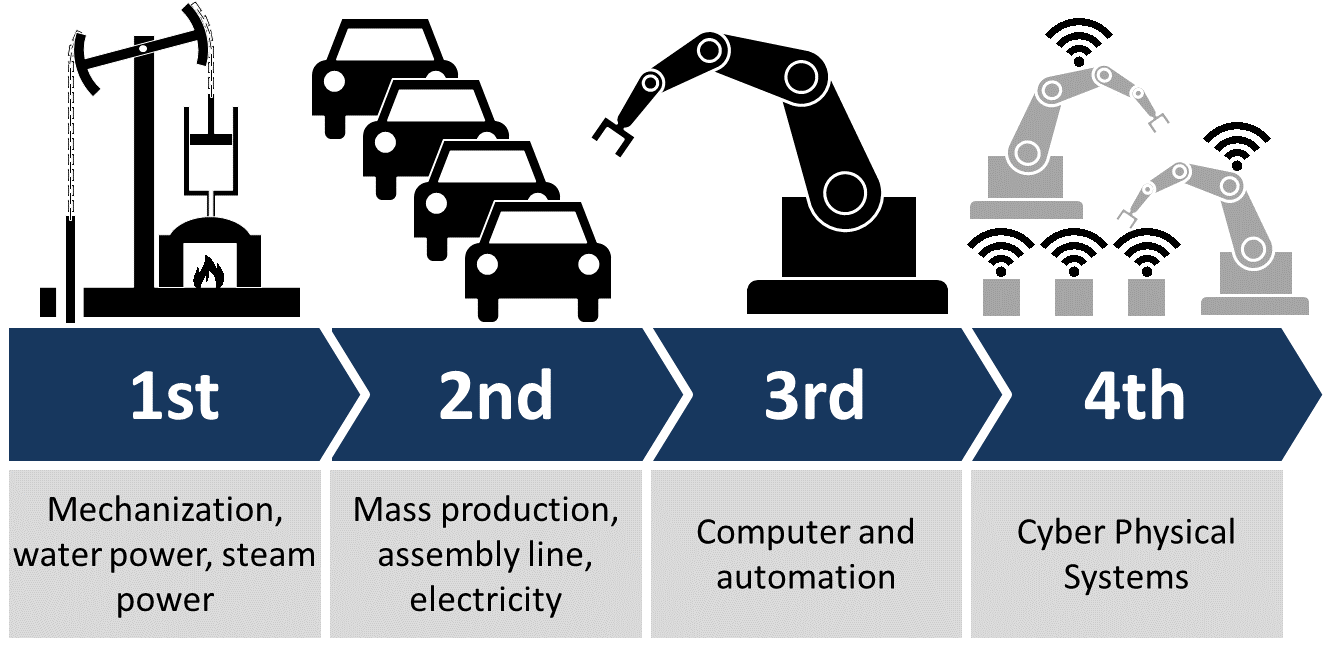
\includegraphics[scale=0.3]{chap1/fig3.png}
\caption{Révolutions industrielles \cite{wan2015industrie}}
\label{fig3}
\end{figure}
\subsection{Environnement}
En déployant des capteurs environnementaux, nous pouvons mesurer et surveiller la qualité de l'air, la qualité de l'eau, les conditions du sol, le rayonnement et les produits chimiques dangereux plus efficacement. Nous pouvons également mieux prévoir les tremblements de terre et les tsunamis et détecter plus rapidement les incendies de forêt, les avalanches de neige et les glissements de terrain. Tout cela nous aidera à mieux protéger notre environnement \cite{cheng2012establishing}. En marquant les animaux sauvages, en particulier les espèces en voie de disparition, nous pouvons étudier et mieux comprendre le comportement des animaux \cite{memon2016internet,nobrega2018animal}, et ainsi offrir une meilleure protection et des habitats plus sûrs. L'IoT permettra également une agriculture intelligente, qui offrira une visibilité 24/7 sur la santé des sols et des cultures, et aidera les agriculteurs à optimiser l'utilisation des engrais et des produits phytopharmaceutiques. Cela aura à nouveau inévitablement un impact positif sur l'environnement \cite{muangprathub2019iot}.
\section{Technologies de communication}
Outre les techniques de communications conventionnelles telles qu’Ethernet, Wi-Fi et Bluetooth, de nombreuses autres technologies peuvent être utilisées pour les communications sur l'Internet des objets.
\subsection{RFID et NFC (Near‐Field Communication)}
L'identification par radiofréquence, en anglais Radio‐frequency identification (RFID) est une technologie qui peut identifier et suivre de manière unique les étiquettes attachées aux objets à l'aide d'ondes électromagnétiques radiofréquence \cite{agrawal2013survey}. Un système RFID comprend généralement une étiquette, un lecteur et une antenne. Le lecteur envoie un signal d'interrogation à l'étiquette via l'antenne, et l'étiquette répond avec ses informations uniques. Les étiquettes RFID peuvent être actives ou passives. Les étiquettes RFID actives ont leur source d'alimentation et peuvent donc être lues sur une longue portée (jusqu'à 100 mètres) \cite{amendola2014rfid}. Les étiquettes RFID passives n'ont pas leur source d'alimentation. Ils sont alimentés par l'énergie électromagnétique transmise par le lecteur RFID. Par conséquent, ils ne peuvent être lus que sur une courte distance (<25m) \cite{jia2012rfid}. La RFID fonctionne principalement dans les gammes de fréquences suivantes, comme indiqué dans Tableau \ref{tab1}.


La communication en champ proche, en anglais Near‐field communication (NFC) est une technologie de communication qui fonctionne à la même fréquence (13,56 MHz) que la RFID HF \cite{al2016comparison}. Différent de la RFID, le NFC est basé sur une communication d'égal à égal, ce qui signifie qu'un appareil NFC peut être soit un lecteur soit une étiquette.


Cette capacité unique a fait du NFC un choix populaire pour le paiement sans contact, les cartes d'identité et les cartes de voyage, etc. Les appareils NFC communiquent généralement à moins de 4 cm (2 pouces) les uns des autres. NFC est désormais disponible sur la plupart des nouveaux smartphones. Les smartphones NFC peuvent être utilisés pour le paiement sans contact, ainsi que pour transmettre les informations (informations de contact ou photographies) d'un smartphone à l'autre en tapant les deux appareils ensemble \cite{shah2016survey}.

\begin{table}[H]
\caption{Bandes de fréquences RFID}
\label{tab1}
\begin{tabular}{|l|l|l|l|}
\hline
\multicolumn{1}{|c|}{\textbf{Band}}                                                    & \multicolumn{1}{c|}{\textbf{Range}} & \multicolumn{1}{c|}{\textbf{Data Speed}} & \multicolumn{1}{c|}{\textbf{Tags}} \\ \hline
Low frequency (LF): 125–134.2 kHz                                                      & 10 m                                & low                                      & passive                            \\ \hline
High frequency (HF): 13.56 MHz                                                         & 10 cm–1 m                           & low to moderate                          & passive                            \\ \hline
Ultra high frequency (UHF): 433 MHz                                                    & 1–100 m                             & moderate                                 & passive or active                  \\ \hline
\begin{tabular}[c]{@{}l@{}}Ultra high frequency (UHF):856 MHz–960\\   MHz\end{tabular} & 1–12 m                              & moderate to high                         & passive or active                  \\ \hline
Microwave:  2.45–5.8 GHz                                                               & 1–2 m                               & high                                     & active                             \\ \hline
Microwave: 3.1–10 GHz                                                                  & \textless{}200 m                    & high                                     & active                             \\ \hline
\end{tabular}
\end{table}
\subsection{Bluetooth Low Energy (BLE)}
Bluetooth low energy (BLE) est un membre plus récent de la famille Bluetooth, basé sur les normes Bluetooth 4.0. Semblable au Bluetooth classique, le BLE fonctionne également dans la bande ISM 2,4 GHz mais utilise un système de modulation plus simple. Le BLE reste constamment en mode veille, sauf lorsqu'une connexion est établie et consomme donc beaucoup moins d'énergie \cite{chang2014bluetooth}.
BLE est arrivé sur le marché en 2011 et est commercialisé sous le nom de Bluetooth Smart. Le BLE est conçu pour fournir une consommation d'énergie et des coûts très réduits tout en conservant une plage de communication similaire. Le BLE fonctionne généralement à une distance d'environ 100 m, avec un débit de données d'environ 1 Mbits/s \cite{teran2017iot}.
Les applications typiques du BLE sont:
\begin{itemize}
    \item Moniteurs de fréquence cardiaque
\item Tensiomètres
\item 	Moniteurs de glycémie
\item 	Appareils Fitbit
\item Capteurs de surveillance industriels
\item 	Promotions ciblées basées sur la géographie (iBeacon)
\item 	Détection de proximité 

\end{itemize}

\subsection{LiFi}
Light Fidelity (LiFi) est une nouvelle technologie de communication haute vitesse sans fil, bidirectionnelle, basée sur la lumière visible à modulation rapide. Il s'agit d'un type de système de communication à lumière visible (Visible Light Communications : VLC). Semblable au WiFi, le LiFi transmet des données à l'aide d'ondes électromagnétiques \cite{haas2018lifi}. Mais au lieu d'utiliser des ondes radio (MHz - GHz), il utilise la lumière visible (~ THz). LiFi utilise des ampoules LED domestiques (light-emitting diodes) comme émetteurs. En faisant varier le courant électrique fourni à une ampoule LED à des vitesses extrêmement élevées, les données peuvent être encodées à mesure que la luminosité change rapidement, qui peuvent ensuite être captées par un photodétecteur (photodiode). Ces changements rapides sont trop rapides pour être remarqués aux yeux des humains; par conséquent, le LiFi n'affecte pas la fonction principale des lumières LED - l'éclairage \cite{haas2015lifi}. 

Le LiFi a un énorme avantage en termes d'infrastructure, car les ampoules LED sont de plus en plus utilisées dans les bâtiments, les rues et les véhicules. Il peut fonctionner à une vitesse impressionnante pouvant atteindre 224 gigabits par seconde et il est insensible aux interférences électromagnétiques. Le LiFi ne peut pas pénétrer les murs, ce qui signifie qu'il ne peut fonctionner qu'à courte portée, mais en même temps, cela le rend moins susceptible d'être piraté. Il existe déjà des produits sur le marché qui peuvent fournir à la fois lumière et connectivité \cite{bokefode2018retrieving}.
\subsection{6LowPAN}
6LoWPAN signifie IPv6 (Internet Protocol Version 6) sur les réseaux personnels sans fil à faible puissance (Personal Area Networks: WPAN) \cite{catarinucci2015iot}. Il s'agit essentiellement d'un réseau maillé sans fil à faible puissance et faible débit basé sur les normes IEEE 802.15.4, utilisant IPv6 comme protocole de communication. Comparé à d'autres réseaux locaux, 6LoWPAN a un avantage distinct, c'est-à-dire qu'il est basé sur des normes ouvertes TCP/IP, y compris TCP, UDP, HTTP, CoAP, MQTT et WebSockets etc \cite{pongle2015survey}. Il a des nœuds adressables IPv6 de bout en bout et peut être facilement connecté à Internet directement. Il est également auto-réparateur en raison du routage du maillage. 6LoWPAN a été utilisé dans les réseaux de capteurs sans fil, les lumières et les compteurs \cite{gomez20176lowpan}.
\subsection{ZigBee}
ZigBee est une technologie de communication de haut niveau pour les réseaux personnels à faible puissance et à faible débit de données, tels que les réseaux de capteurs \cite{feng2008zigbee}, les automatismes domestiques et les dispositifs médicaux. ZigBee est basé sur la norme IEEE 802.15.4. Il a une distance de transmission de 10 à 100 mètres et doit être en ligne de mire. Il opère dans les bandes radio industrielles, scientifiques et médicales (ISM), à savoir 868 MHz en Europe, 915 MHz aux États-Unis et en Australie, 784 MHz en Chine et 2,4 GHz dans le reste du monde \cite{markovtechnical}. ZigBee a un débit de données allant de 20 kbit / s (bande 868 MHz) à 250 kbit / s (bande 2,4 GHz). Les réseaux ZigBee sont normalement moins chers que les autres réseaux sans fil tels que Bluetooth ou WiFi. ZigBee a été utilisé pour les interrupteurs d'éclairage sans fil, les compteurs électriques (réseau intelligent, réponse à la demande, etc.), la surveillance des équipements industriels, etc \cite{hasan1999intelligent}.


La différence entre ZigBee et 6LoWPAN, ZigBee a été plus longtemps, et a donc été adopté plus largement que 6LoWPAN \cite{lu2011interconnecting}. ZigBee est sans aucun doute la norme de réseautique maillée sans fil à faible coût et à faible consommation d'énergie la plus populaire actuellement. Cependant, 6LoWPAN rattrape son retard et devient plus attractif, car il est basé sur IP, en particulier avec le support IPv6. Cela facilite l'intégration avec le reste d'Internet. À ce jour, de nombreuses sociétés de semi-conducteurs (par exemple, Texas Instruments, Freescale et Atmel, etc.) fabriquent des puces 802.15.4 qui prennent en charge à la fois ZigBee et 6LoWPAN \cite{drake2014zigbee}.
\subsection{Z‐Wave}
Z-Wave est une technologie de communication sans fil qui est principalement utilisée pour la domotique, comme le contrôle et l'automatisation des lumières et des appareils. Il peut être utilisé comme système de sécurité ou pour surveiller et contrôler votre propriété à distance \cite{unwala2018iot}. Z-Wave fonctionne dans la bande industrielle, scientifique et médicale (ISM) non autorisée, à savoir 868,42 MHz en Europe, 908,42 MHz aux États-Unis et au Canada, et d'autres fréquences dans d'autres régions. Z-Wave est conçu pour fournir une transmission fiable à faible latence à une portée d'environ 100 mètres, avec des débits de données jusqu'à 100 kbit/s. Un réseau Z-Wave comprend normalement un contrôleur principal et une collection de périphériques (jusqu'à 232) \cite{unwala2017iot}.

\subsection{LoRa}

LoRa est une technologie de communication à longue portée conçue pour les communications à faible puissance et à longue distance des dispositifs IoT alimentés par batterie, c'est-à-dire un réseau étendu à faible puissance (LPWAN). Il prend en charge les communications bidirectionnelles sécurisées des réseaux avec des millions et des millions d'appareils \cite{vangelista2015long,vejlgaard2017coverage}.


Le tableau \ref{tabcom}  présente une comparaison rapide des différentes technologies de communication sans fil. Le LiFi et le WiFi offrent potentiellement les débits de données les plus élevés, tandis que le cellulaire et le LoRa offrent les plus longues distances.

\begin{table}[H]

\caption{Comparaison de différentes technologies}
\label{tabcom}
\begin{tabular}{lllll}

\hline
\multicolumn{1}{|c|}{\textbf{}} & \multicolumn{1}{c|}{\textbf{Standard}}                                                                                & \multicolumn{1}{c|}{\textbf{Frequency}}                                                                                               & \multicolumn{1}{c|}{\textbf{Range}}    & \multicolumn{1}{c|}{\textbf{Data Rate}}                                                                                                                                    \\ \hline
\multicolumn{1}{|l|}{LiFi}      & \multicolumn{1}{l|}{Similar to 802.11}                                                                                & \multicolumn{1}{l|}{400–800 THz}                                                                                                      & \multicolumn{1}{l|}{\textless{}10 m}   & \multicolumn{1}{l|}{\textless{}224 Gbps}                                                                                                                                   \\ \hline
\multicolumn{1}{|l|}{WiFi}      & \multicolumn{1}{l|}{802.11a/b/g/n/ac}                                                                                 & \multicolumn{1}{l|}{2.4 GHz and 5 GHz}                                                                                                & \multicolumn{1}{l|}{$\sim$50 m}        & \multicolumn{1}{l|}{\textless{}1 Gbps}                                                                                                                                     \\ \hline
\multicolumn{1}{|l|}{Cellular}  & \multicolumn{1}{l|}{\begin{tabular}[c]{@{}l@{}}GSM/GPRS/EDGE\\   (2G), UMTS/HSPA\\   (3G), LTE (4G), 5G\end{tabular}} & \multicolumn{1}{l|}{\begin{tabular}[c]{@{}l@{}}900, 1800, 1900, and\\   2100MHz\\   2.3, 2.6, 5.25, 26.4, and 58.68 GHz\end{tabular}} & \multicolumn{1}{l|}{\textless{}200 km} & \multicolumn{1}{l|}{\begin{tabular}[c]{@{}l@{}}\textless{}500 kps (2G),\\   \textless{}2 Mbps (3G),\\   \textless{}10 Mbps (4G)\\   \textless{}100 Mbps (5G)\end{tabular}} \\ \hline
\multicolumn{1}{|l|}{Bluetooth} & \multicolumn{1}{l|}{Bluetooth 4.2}                                                                                    & \multicolumn{1}{l|}{2.4 GHz}                                                                                                          & \multicolumn{1}{l|}{50–150 m}          & \multicolumn{1}{l|}{1 Mbps}                                                                                                                                                \\ \hline
\multicolumn{1}{|l|}{RFID/NFC}  & \multicolumn{1}{l|}{ISO/IEC 18000‐3}                                                                                  & \multicolumn{1}{l|}{13.56 MHz}                                                                                                        & \multicolumn{1}{l|}{10 cm}             & \multicolumn{1}{l|}{100–420 kbps}                                                                                                                                          \\ \hline
\multicolumn{1}{|l|}{6LowPAN}   & \multicolumn{1}{l|}{RFC6282}                                                                                          & \multicolumn{1}{l|}{2.4 GHz and $\sim$1 GHz}                                                                                          & \multicolumn{1}{l|}{\textless{}20 m}   & \multicolumn{1}{l|}{20–250 kbps}                                                                                                                                           \\ \hline
\multicolumn{1}{|l|}{ZigBee}    & \multicolumn{1}{l|}{\begin{tabular}[c]{@{}l@{}}ZigBee 3.0 based on\\   IEEE 802.15.4\end{tabular}}                    & \multicolumn{1}{l|}{2.4 GHz}                                                                                                          & \multicolumn{1}{l|}{10–100 m}          & \multicolumn{1}{l|}{250 kbps}                                                                                                                                              \\ \hline
\multicolumn{1}{|l|}{Z‐Wave}    & \multicolumn{1}{l|}{\begin{tabular}[c]{@{}l@{}}Z‐Wave Alliance\\   ZAD12837 / ITU‐T\\   G.9959\end{tabular}}          & \multicolumn{1}{l|}{\begin{tabular}[c]{@{}l@{}}868.42 MHz and\\   908.42 MHz\end{tabular}}                                            & \multicolumn{1}{l|}{\textless{}100 m}  & \multicolumn{1}{l|}{\textless{}100 kbps}                                                                                                                                   \\ \hline
\multicolumn{1}{|l|}{LoRa}& \multicolumn{1}{l|}{LoRaWAN}                                                                                                               & \multicolumn{1}{l|}{868 MHz and 915 MHz }                                                                                                                  & \multicolumn{1}{l|}{\textless{}15 km  }                     & \multicolumn{1}{l|}{0.3–50 kbps    }                                 \\ \hline                                                                                                            
\end{tabular}
\end{table}
\section{Protocoles de l'internet des objets}
Les protocoles, ou les protocoles de communication, sont un ensemble de règles qui permettent aux appareils de communiquer entre eux. Les protocoles définissent la syntaxe, la sémantique et la synchronisation de la communication. Une analogie étroite avec les protocoles est celle des langues humaines. Il existe de nombreux protocoles de communication disponibles pour les applications IoT. Les protocoles suivants sont couramment utilisés: HTTP, Websocket et MQTT.
\subsection{Hypertext Transfer Protocol}
Le protocole de transfert hypertexte (Hypertext Transfer Protocol : HTTP) est le protocole de communication derrière le World Wide Web (WWW). Il est basé sur une architecture client-serveur et fonctionne à la manière des demandes et des réponses. HTTP utilise TCP (protocole de contrôle de transmission) pour fournir des connexions fiables \cite{yokotani2016comparison}.


HTTP est un protocole sans état, car le client et le serveur ne maintiennent pas de connexion pendant la communication. La version actuelle est HTTP/1.1 et la version précédente est HTTP/1.0. La nouvelle version HTTP/2 arrive bientôt, qui aura de nombreuses nouvelles fonctionnalités, telles que la poussée du serveur, pour minimiser le nombre de demandes des clients et augmenter la vitesse \cite{daud2016internet}.

\subsection{WebSocket}
WebSocket est un protocole de communication conçu pour les navigateurs Web et les serveurs Web, mais contrairement à HTTP, WebSocket fournit une communication en duplex intégral sur une seule connexion TCP. WebSocket est avec état, car le client et le serveur maintiennent une connexion pendant la communication. Le WebSocket permet une plus grande interaction entre un navigateur et un serveur Web, permet un transfert de données en temps réel et des flux de messages. À ce jour, WebSocket est implémenté dans tous les principaux navigateurs Web, par exemple Firefox 6, Safari 6, Google Chrome 14, Opera 12.10 et Internet Explorer 10 \cite{longo2017stack4things,seo2018design}.
\subsection{MQ Telemetry transport (MQTT)}
MQ Telemetry transport (MQTT) est un protocole de communication machine à machine légère conçue pour les appareils IoT par IBM. MQTT est basé sur un modèle publisher-subscriber, où publisher publie des données sur un serveur (également appelé broker), et le subscriber s'abonne au serveur et reçoit des données du serveur. Le broker MQTT est responsable de la distribution des messages et peut-être quelque part dans le Cloud \cite{lampkin2012building,yassein2017internet}. 
\subsection{Constrained application Protocole (CoAP)}
Constrained application Protocole (CoAP)  est un protocole de couche application spécialisé pour les dispositifs IoT contraints, c'est-à-dire les devices avec une puissance de calcul, une consommation d'énergie et une connectivité réseau limitée \cite{shelby2014constrained}, etc. Il est basé sur des messages de demande et de réponse, similaires à HTTP, mais il utilise UDP (user datagram protocole) plutôt TCP (transmission contrôle protocole). Bien que UDP ne fournisse pas de transmissions fiables, il est beaucoup plus simple, à un sur débit beaucoup plus petit, et donc il est beaucoup plus rapide. CoAP est conçu pour les applications de machine à machine (M2 M) telles que l'énergie intelligente et l'automatisation de la maison/du bâtiment building automation \cite{bormann2012coap}.
\subsection{Extensible Messaging and Presence Protocol (XMPP)}
Extensible Messaging and Presence Protocol (XMPP) est un protocole de communication en temps réel standard ouvert basé sur XML (Extensible Markup Language). Il peut fournir une large gamme de services, notamment la messagerie instantanée, la présence et la collaboration. Il est décentralisé et dispose de fonctions de sécurité. Il est également extensible, ce qui signifie qu'il est conçu pour grandir et s'adapter aux changements. Le logiciel XMPP comprend des serveurs, des clients et des bibliothèques \cite{saint2004extensible,bendel2013service}.
\section{Système embarqué}
Le premier système informatique embarqué moderne en temps réel a été l'ordinateur de guidage Apollo, développé dans les années 1960 par le Dr Charles Stark Draper au Massachusetts Institute of Technology pour le programme Apollo. L'ordinateur de guidage Apollo a été conçu pour collecter automatiquement des données et fournir des calculs critiques pour le module de commande Apollo et le module lunaire.

En 1971, Intel a sorti la première unité de microprocesseur disponible dans le commerce - l'Intel 4004 - un premier microprocesseur qui nécessitait encore des puces de support et une mémoire externe; en 1978, la National Engineering Manufacturers Association a publié une norme pour les microcontrôleurs programmables, améliorant la conception du système embarqué; et au début des années 80, les composants du système de mémoire, d'entrée et de sortie avaient été intégrés dans la même puce que le processeur, formant un microcontrôleur.

Le système intégré basé sur un microcontrôleur continuerait d’être intégré dans tous les aspects de la vie quotidienne des consommateurs, des lecteurs de cartes de crédit et des téléphones portables aux feux de circulation et aux thermostats.
\subsection{Définition du système embarqué}

Un système embarqué est un système informatique à petite échelle qui fait partie d'une machine ou d'un système électrique/mécanique plus grand. Il est souvent conçu pour effectuer certaines tâches dédiées et souvent un système en temps réel. Il est appelé intégré car le système informatique est intégré à un périphérique matériel. Les systèmes intégrés sont importants, car ils sont de plus en plus utilisés dans de nombreux appareils quotidiens \cite{pavithra2015iot}, tels que les montres numériques, les appareils photo, les fours à micro-ondes, les machines à laver, les chaudières, les réfrigérateurs, les téléviseurs intelligents et les voitures. Les systèmes embarqués doivent également souvent être de petite taille, à faible coût et avoir une faible consommation d'énergie \cite{samie2016iot}.

Un système embarqué comprend trois composants:
\begin{itemize}
    \item Le matériel.

  \item Un logiciel d'application.

  \item Il dispose d'un système d'exploitation en temps réel (SETR) qui supervise le logiciel d'application et fournit un mécanisme permettant au processeur d'exécuter un processus conformément au calendrier en suivant un plan de contrôle des latences. SETR définit le fonctionnement du système. Il définit les règles lors de l'exécution du programme d'application. Un système intégré à petite échelle peut ne pas avoir de SETR.


\end{itemize}

Nous pouvons donc définir un système embarqué comme un système de contrôle en temps réel basé sur un microcontrôleur, piloté par logiciel et fiable.


La figure \ref{fig4} montre le diagramme schématique d'un système embarqué typique qui comprend un microcontrôleur, des entrées/sorties et des interfaces de communication.
\begin{figure}[H]
\centering
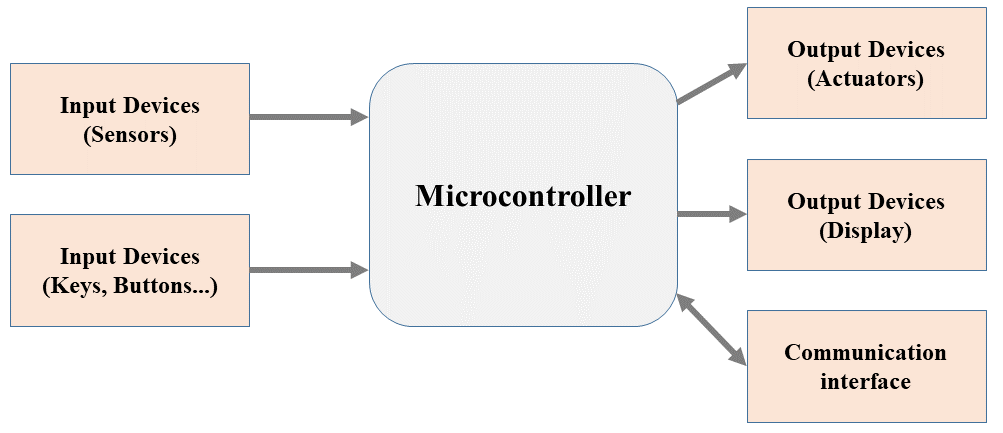
\includegraphics[scale=0.5]{chap1/Presentation21.png}
\caption{Diagramme schématique d'un système embarqué typique}
\label{fig4}
\end{figure}
\subsubsection{Microcontroller}
Le microcontrôleur est le cerveau d'un système embarqué, qui orchestre toutes les opérations. Un microcontrôleur est un processeur d'ordinateur avec la mémoire et tous les périphériques d'entrée/sortie. Plus de détails sur les microcontrôleurs seront illustrés dans la section suivante.
\subsubsection{Les entrées}
Un système embarqué interagit avec le monde extérieur via ses entrées et sorties. Les entrées peuvent être des entrées numériques ou des entrées analogiques. Les entrées sont généralement utilisées pour lire les données des capteurs (capteur de température, capteur de lumière, capteur à ultrasons, etc.) ou d'autres types de périphériques d'entrée (touches, boutons, etc...).
\subsubsection{Les sorties}
Les sorties peuvent également être des sorties numériques ou des sorties analogiques. Les sorties sont généralement utilisées pour l'affichage, la commande de moteurs ou d'autres dispositifs (actionneurs).
\subsubsection{Interfaces de communication}
Un système embarqué communique avec d'autres appareils à l'aide d'interfaces de communication, notamment Ethernet, USB (Universal Serial Bus), CAN (Controller Area Network), infrarouge, ZigBee, WiFi et Bluetooth.

\subsection{Caractéristiques d'un système embarqué}
les systèmes embarqués se caractérisent par:
\begin{itemize}
    \item \textbf{Fonction unique:} un système embarqué effectue généralement une opération spécialisée et fait de même à plusieurs reprises. Par exemple, un téléavertisseur fonctionne toujours comme un téléavertisseur.
    
    
    \item \textbf{Contraintes strictes:} tous les systèmes informatiques ont des contraintes sur les métriques de conception, mais celles d'un système embarqué peuvent être particulièrement strictes. Les métriques de conception sont une mesure des fonctionnalités d'une implémentation telles que son coût, sa taille, sa puissance et ses performances. Il doit être d'une taille adaptée à une seule puce, doit être suffisamment rapide pour traiter les données en temps réel et consommer un minimum d'énergie pour prolonger la durée de vie de la batterie.
    \item \textbf{Réactif et en temps réel:} de nombreux systèmes embarqués doivent constamment réagir aux changements de l'environnement du système et doivent calculer certains résultats en temps réel sans aucun délai. Prenons un exemple de régulateur de vitesse pour voiture; il surveille et réagit en permanence aux capteurs de vitesse et de freinage. Il doit calculer à plusieurs reprises l'accélération ou les des accélérations dans un temps limité; un calcul retardé peut entraîner un échec de contrôle de la voiture.
    \item \textbf{Basé sur des microprocesseurs:} il doit être basé sur un microprocesseur ou un microcontrôleur.
    \item \textbf{Mémoire:} il doit avoir une mémoire, car son logiciel est généralement intégré dans la ROM. Il n'a pas besoin de mémoire secondaire sur l'ordinateur.
    \item \textbf{Connecté:} il doit avoir des périphériques connectés pour connecter les périphériques d'entrée et de sortie.
    \item \textbf{Systèmes matériels / logiciels:} le logiciel est utilisé pour plus de fonctionnalités et de flexibilité. Le matériel est utilisé pour les performances et la sécurité.
\end{itemize}
\subsection{Structure de base d'un système embarqué}
L'illustration suivante montre la structure de base d'un système embarqué 

\begin{figure}[H]
    \centering
    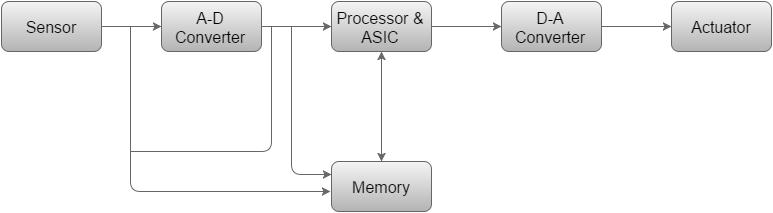
\includegraphics[scale=0.6]{chap1/embedded_systems_structure.jpg}
    \caption{Structure de base d'un système embarqué}
    \label{fig:se}
\end{figure}
\begin{itemize}
    \item \textbf{Capteur:} il mesure la quantité physique et la convertit en un signal électrique qui peut être lu par un observateur ou par n'importe quel instrument électronique comme un convertisseur A2D. Un capteur stocke la quantité mesurée dans la mémoire.

\item \textbf{Convertisseur A-D:} un convertisseur analogique-numérique convertit le signal analogique envoyé par le capteur en un signal numérique.

\item \textbf{Processeur et ASIC:} les processeurs traitent les données pour mesurer la sortie et les stockent dans la mémoire.

\item \textbf{Convertisseur D-A:} un convertisseur numérique-analogique convertit les données numériques fournies par le processeur en données analogiques

\item \textbf{Actionneur:} un actionneur compare la sortie donnée par le convertisseur D-A à la sortie réelle (attendue) qui y est stockée et stocke la sortie approuvée.
\end{itemize}
\subsection{Tendances futures des systèmes embarqués}
L'industrie des systèmes embarqués devrait continuer de croître rapidement, tirée par le développement continu de l'intelligence artificielle (IA), de la réalité virtuelle (VR) et de la réalité augmentée (AR), de l'apprentissage automatique, de l'apprentissage en profondeur et de l'Internet des objets (IoT).

Le système embarqué cognitif sera au cœur de tendances telles que la réduction de la consommation d'énergie, l'amélioration de la sécurité des appareils embarqués, la connectivité cloud et la mise en réseau maillée, les applications d'apprentissage en profondeur et les outils de visualisation avec des données en temps réel.
\section{Conclusion}
Dans ce chapitre nous avons fait un survol sur l’internet des objets en général en fournissant la définition d'un objet connecté, de son architecture et de l’architecture de l'IoT. On a vu aussi l’historique de l'IoT et les raisons de cette évolution. Ensuite on a expliqué les technologies et les domaines d’application qui seront touchés par l’émergeant d’internet des objets ainsi que les défis et comment appliquer le système embarqué.


 Dans le chapitre suivant, nous allons présenter dans la première section l'historique du cloud computing, ses propres définitions, leur caractéristiques , ses services et les modèles de déploiement de cloud computing, enfin nous allons cité quelques avantages et inconvénients de cloud computing.





